% !TeX spellcheck = en_US
% !TEX root = ../thesis-example.tex
%
\chapter{Extending Reality}
\label{sec:extendingreality}

\cleanchapterquote{You are an aperture through which the universe is looking at 
and exploring itself.}{Alan W. Watts}{(Philosopher)}

The well known urban legend of "L'Arriv\'ee d'un train en gare de La Ciotat" in 
which a train arrives at the La Ciotat station, is, that "the audience was so 
overwhelmed by the moving image [...] coming directly at them that people 
screamed and ran to the back of the room". \cite{wiki:train:2017} With that a 
new medium was created, which matured into a new art form of film and movies.
\todo[inline]{This sounds more like prosa text.}

\section{Motion Video Production}

Producing motion video has come a long way and a sufficient history of it would 
be far out of scope of this thesis. Concentrating on key aspects of composition 
techniques might give an appropriate overview to range where Mixed Reality 
takes its inspiration from.

Way before digital imaging processing took over production sets similar 
problems as discussed in this thesis had to be solved, i. e. how an actor can 
be captured without a back- or foreground and how he would then be integrated 
into an imaginative set. Today, modern action movies don't even necessarily 
capture the actor but his movements, which then will be artificially rendered 
with computer generated imagery.

\section{CGI \& Video Composition}

\subsection{History of Green \& Blue Screen Productions}

Set theory is beyond the scope of this thesis, but green- and blue screen 
production has first and foremost a simple reasoning: Green and blue are two of 
the three color triplets that resemble a least amount of color of humans - and 
to a certain extent any flora and fauna. Since chroma keying (see Ch. 
\ref{sec:chromakey}) takes color distance as general basis, production 
environments generally use green screen keying.
\newline
Greenscreens abuse a correlating advantage that the human eye is most 
susceptible to green, allowing for a visual high color range and an ability to 
differentiate between many shades of green. Experiments to color range have 
been done since 1942, trying to understand color ranges and color difference of 
human vision. Experiments conclude that eye cone cells see a blending range of 
wavelengths to different intensities, giving the green vector space its highest 
range. \cite{MacAdam:1942}

\begin{figure}[htbp]
	\label{fig:greenscreen:stimula}
	\begin{subfigure}[t]{.35\textwidth}
		\centering
		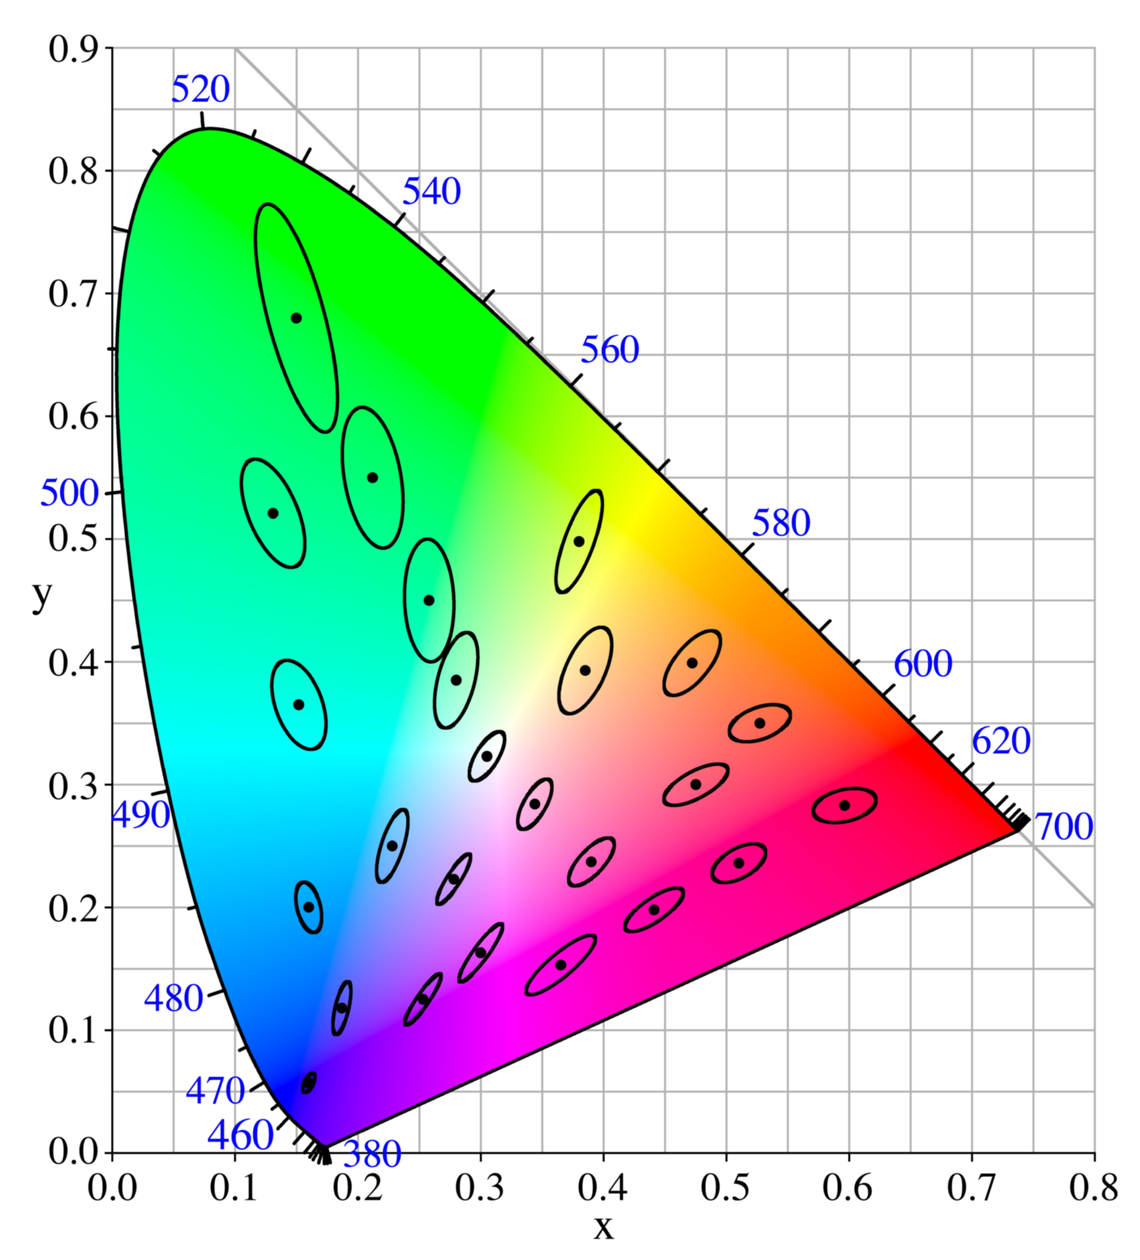
\includegraphics[width=\textwidth]{_external/media/CIExy1931_MacAdam.png}
	\caption{MacAdam ellipses on 1931 standard chromaticity diagram 
		\cite{wiki:macadam:2017}}
	\end{subfigure}
	\begin{subfigure}[t]{.5\textwidth}
		\centering
		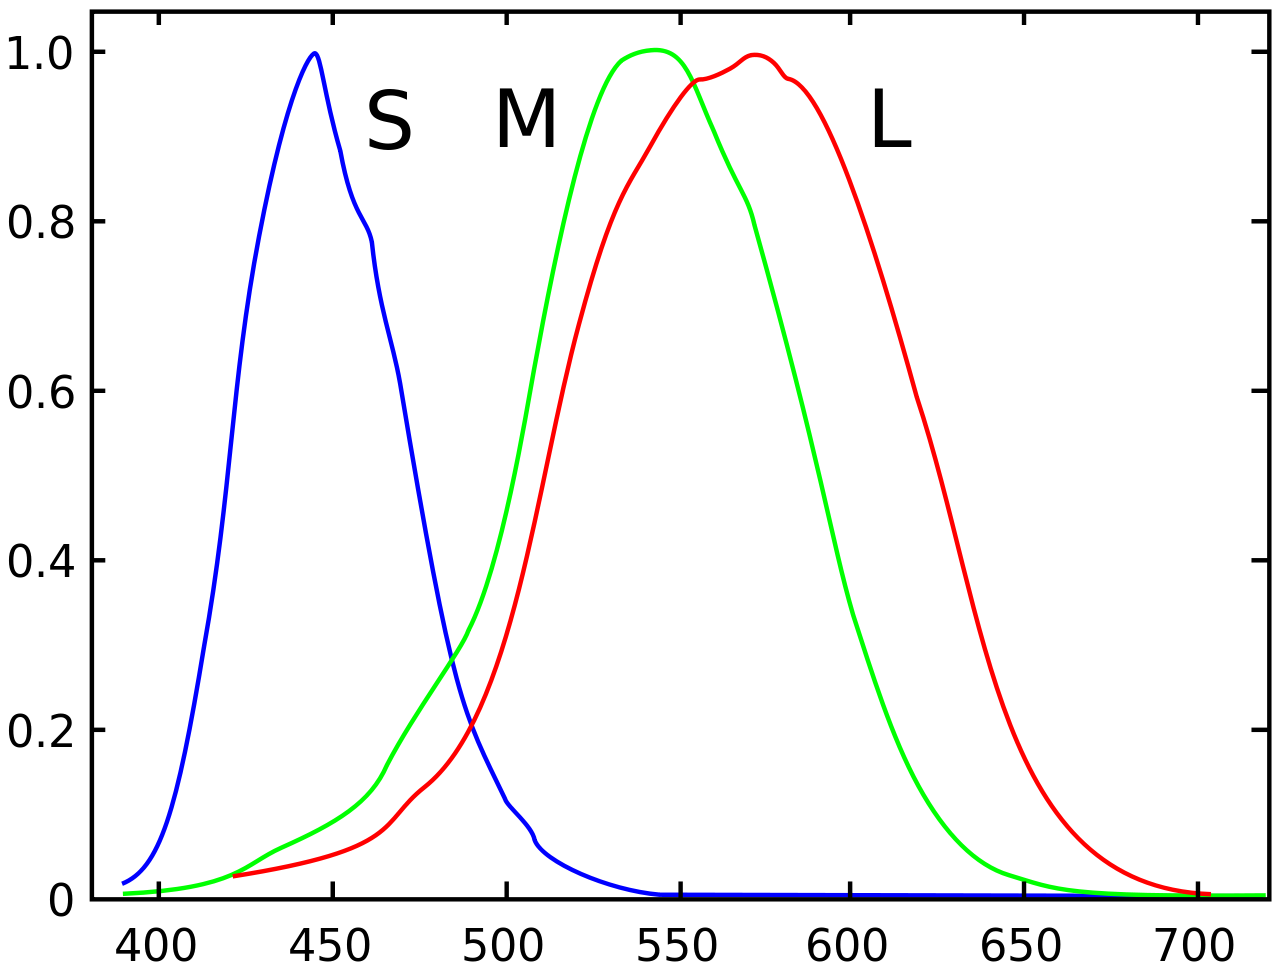
\includegraphics[width=\textwidth]{_external/media/1280px-Cones_SMJ2_E.png}
		\caption{Normalized responsivity spectra of human cone cells, S, M, and 
		L types after Wyszecki et. al \cite{wiki:Wyszecki:2017}}
	\end{subfigure}
\end{figure}

\todo[inline]{The layout is a bit wonky here.}

Most consumer cameras - and even production cameras - use dot-matrix sensors 
with a weighted ration of green (4), red (2) and blue (2) pixels, called Bayer 
pattern \cite{kodak:bayer:1976}. Green is generally easier to light, illuminate 
and adjust over blue 
screens. Small irregularities, for example through uneven lightning or 
crinkles, can be adjusted easily by the user and allows for a 
relatively clean camera image.

\section{What's VR - Differentiation of AR, VR \& MR}

In search of an appropriate abbreviation for computer-enhanced realtime imagery 
a recent addition is "XR", where \textit{X} is a letter of your choice. 
Definitions are getting more diluted and generally describe a technique, rather 
than an apparent effect by now.

\begin{figure}[htb]
	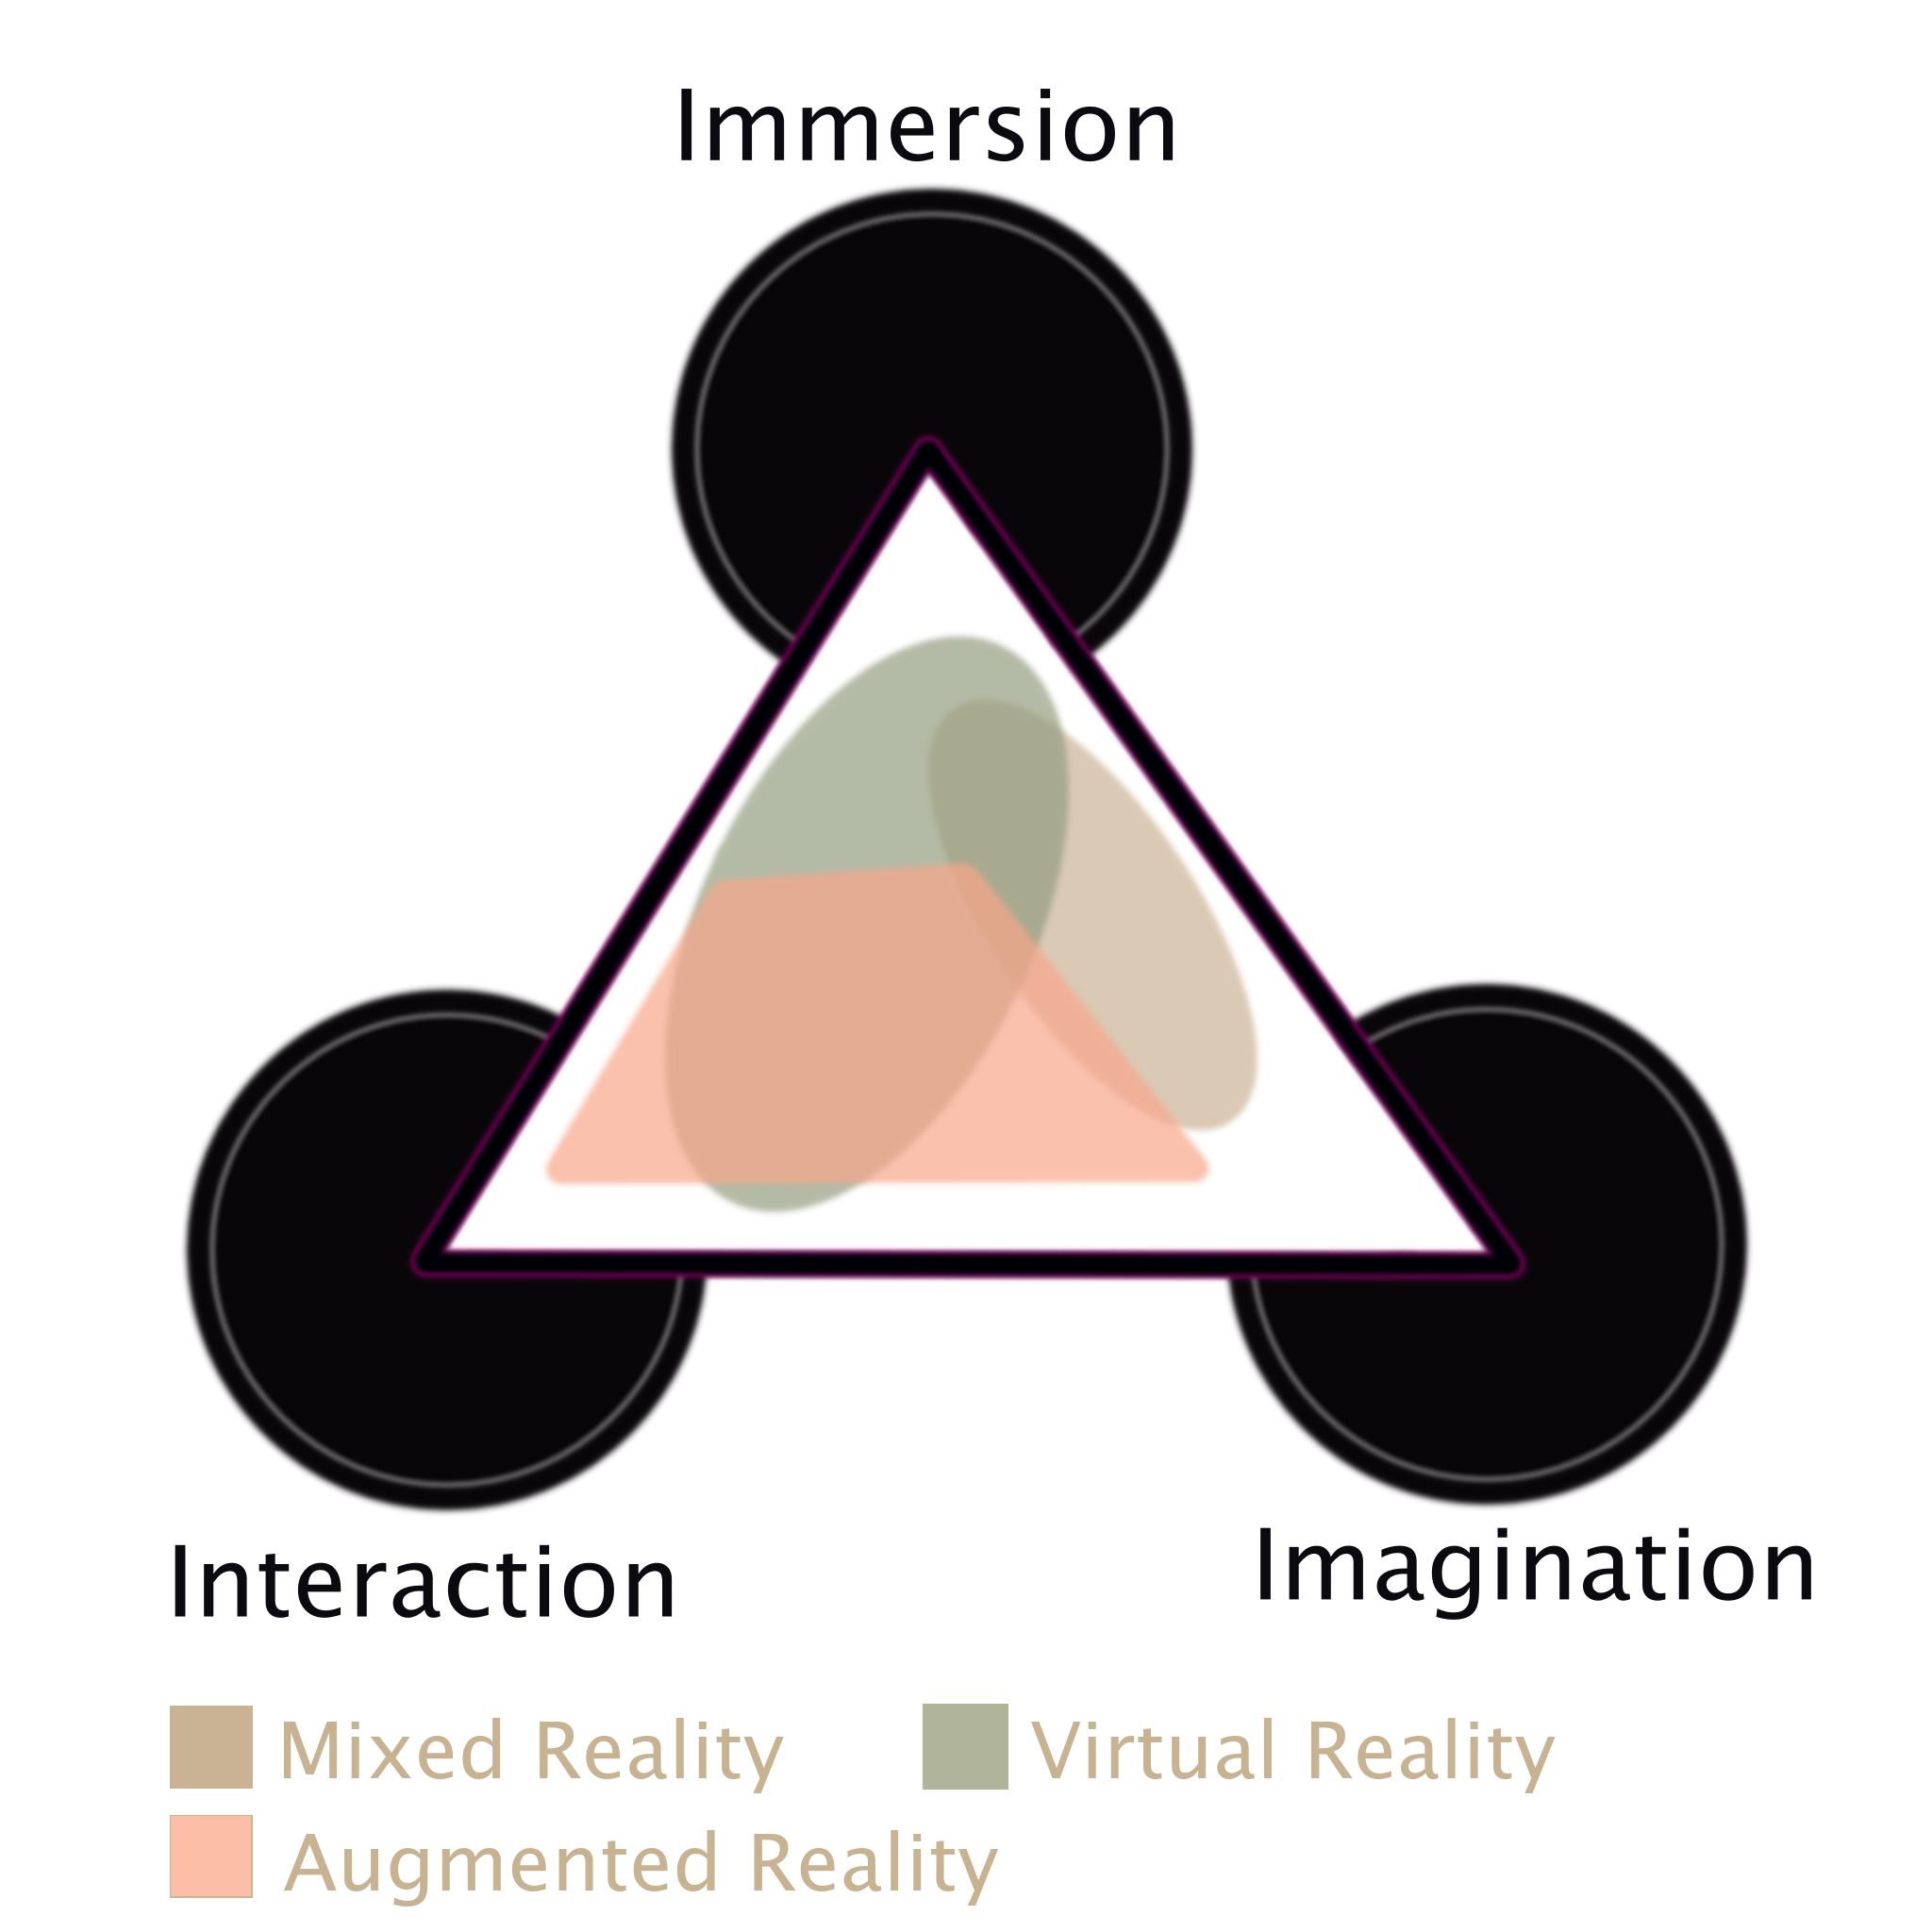
\includegraphics[width=\textwidth]{_raw_resources/i3-triangle.png}
	\caption{I\textsuperscript{3} Triangle - figurative quantization of 
		different reality extending methods}
	\label{fig:xr:i3-triangle}
\end{figure}
Augmented Reality is a concept to augment real world imagery with additional 
information. It ranges from very simple devices displaying data in the field of 
view of the user up to full augmentation, displaying 3D models overlayed of 
real world objects. This can be done ranging from Pepper's Ghost projections, 
to augmenting video - a famous example is the rather successful "Pokémon GO" -, 
up to the Microsoft HoloLens, that has sensors for a wide range of spatial 
mapping, spatial anchoring and distance calculation.

Virtual Reality is usually done by stereo projection of a 3D environment on a 
Head Mounted Display. It takes a user out of the current room and puts him into 
a complete new, virtual reality. Its hardware ranges from the simplistic Google 
Cardboard to the Samsung GearVR up to the Oculus Rift and HTC Vive. The latter 
two products offer room-scale experiences where a user is able to move freely 
in his play space (basically a bounding box) and allows for six degrees of 
freedom (\gls{6dof}) tracking.

Mixed Reality is an extension of Virtual Reality, allowing bystanders to get an 
impression of the virtual reality around an actor. By reproducing virtual 
projection parameters of a 3D environment, it is possible to place a real world 
camera feed at the right position inside the 3D application. This yields to a 
combined technique of Augmented and Virtual Reality. A production environment 
can be achieved with a \gls{6DOF} HMD and additional - either user- or tracking 
input of - positional parameters for the camera. 

\section{Immersion vs. Communication}

\todo[inline]{maybe the overview does already a "good enough" job to bring this 
across.}

Virtual Reality, as previously mentioned in \ref{sec:intro:outline}, is very 
immersive but the experience is hard to imagine without wearing a HMD yourself. 
Additionally doesn't VR offer any ways to allow observers a similar experience 
as the VR actor.
\newline
A very obvious problem starts on interaction. A VR user doesn't always need to 
see his hands to interact with a scene, due to the natural way of holding these 
controllers in his hands and directly translating to interaction inside the 
virtual reality scene. An outside viewer however does not see hands and will 
not understand actions performed by the user. Any usage context that happens 
off-screen cannot be communicated and therefore will be lost.
\newline
A recent game example, Rick and Morty: Virtual Rick-ality, tries to mitigate 
this issue by placing virtual CCTV cameras into the scene, which can be 
controlled through bystanders - giving a neutral third-person view into the 
three-dimension scene. The VR actor is replaced as a loose avatar representing 
a figure (Morty) from the cartoons universe.
\newline
Mixed Reality merges the actors and virtual realities context, allowing outside 
viewers a comparable window into the actors experienced world. In fact, initial 
promotional material for the HTC Vive showed mixed reality footage, produced by 
one VR computer and a secondary composition PC \cite{valve:mr-production:2016}. 
It's setup is comparable to the 
one in this thesis and differs by using more than one software context.

\subsection{Evolution of Virtual Reality Footage}

\section{Mixed Reality and its use cases}

\todo[inline]{Summarize.}

